% Generated by Sphinx.
\def\sphinxdocclass{report}
\documentclass[a4paper,12pt,english]{sphinxmanual}
\usepackage[utf8]{inputenc}
\DeclareUnicodeCharacter{00A0}{\nobreakspace}
\usepackage[T1]{fontenc}
\usepackage{babel}
\usepackage{times}
\usepackage[Bjarne]{fncychap}
\usepackage{longtable}
\usepackage{sphinx}
\usepackage{multirow}


\title{Shakespeare Oracle}
\date{January 20, 2012}
\release{0.3.7}
\author{}
\newcommand{\sphinxlogo}{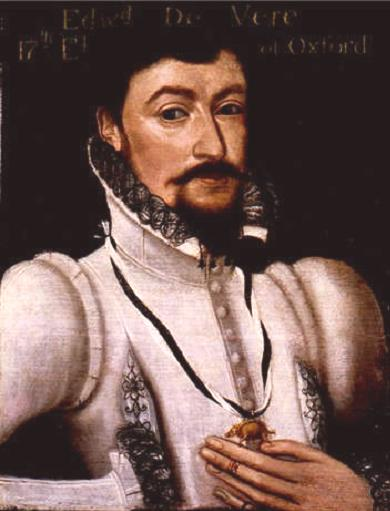
\includegraphics{Edward_de_Vere.JPG}\par}
\renewcommand{\releasename}{Release}
\makeindex

\makeatletter
\def\PYG@reset{\let\PYG@it=\relax \let\PYG@bf=\relax%
    \let\PYG@ul=\relax \let\PYG@tc=\relax%
    \let\PYG@bc=\relax \let\PYG@ff=\relax}
\def\PYG@tok#1{\csname PYG@tok@#1\endcsname}
\def\PYG@toks#1+{\ifx\relax#1\empty\else%
    \PYG@tok{#1}\expandafter\PYG@toks\fi}
\def\PYG@do#1{\PYG@bc{\PYG@tc{\PYG@ul{%
    \PYG@it{\PYG@bf{\PYG@ff{#1}}}}}}}
\def\PYG#1#2{\PYG@reset\PYG@toks#1+\relax+\PYG@do{#2}}

\def\PYG@tok@gd{\def\PYG@tc##1{\textcolor[rgb]{0.63,0.00,0.00}{##1}}}
\def\PYG@tok@gu{\let\PYG@bf=\textbf\def\PYG@tc##1{\textcolor[rgb]{0.50,0.00,0.50}{##1}}}
\def\PYG@tok@gt{\def\PYG@tc##1{\textcolor[rgb]{0.00,0.25,0.82}{##1}}}
\def\PYG@tok@gs{\let\PYG@bf=\textbf}
\def\PYG@tok@gr{\def\PYG@tc##1{\textcolor[rgb]{1.00,0.00,0.00}{##1}}}
\def\PYG@tok@cm{\let\PYG@it=\textit\def\PYG@tc##1{\textcolor[rgb]{0.25,0.50,0.56}{##1}}}
\def\PYG@tok@vg{\def\PYG@tc##1{\textcolor[rgb]{0.73,0.38,0.84}{##1}}}
\def\PYG@tok@m{\def\PYG@tc##1{\textcolor[rgb]{0.13,0.50,0.31}{##1}}}
\def\PYG@tok@mh{\def\PYG@tc##1{\textcolor[rgb]{0.13,0.50,0.31}{##1}}}
\def\PYG@tok@cs{\def\PYG@tc##1{\textcolor[rgb]{0.25,0.50,0.56}{##1}}\def\PYG@bc##1{\colorbox[rgb]{1.00,0.94,0.94}{##1}}}
\def\PYG@tok@ge{\let\PYG@it=\textit}
\def\PYG@tok@vc{\def\PYG@tc##1{\textcolor[rgb]{0.73,0.38,0.84}{##1}}}
\def\PYG@tok@il{\def\PYG@tc##1{\textcolor[rgb]{0.13,0.50,0.31}{##1}}}
\def\PYG@tok@go{\def\PYG@tc##1{\textcolor[rgb]{0.19,0.19,0.19}{##1}}}
\def\PYG@tok@cp{\def\PYG@tc##1{\textcolor[rgb]{0.00,0.44,0.13}{##1}}}
\def\PYG@tok@gi{\def\PYG@tc##1{\textcolor[rgb]{0.00,0.63,0.00}{##1}}}
\def\PYG@tok@gh{\let\PYG@bf=\textbf\def\PYG@tc##1{\textcolor[rgb]{0.00,0.00,0.50}{##1}}}
\def\PYG@tok@ni{\let\PYG@bf=\textbf\def\PYG@tc##1{\textcolor[rgb]{0.84,0.33,0.22}{##1}}}
\def\PYG@tok@nl{\let\PYG@bf=\textbf\def\PYG@tc##1{\textcolor[rgb]{0.00,0.13,0.44}{##1}}}
\def\PYG@tok@nn{\let\PYG@bf=\textbf\def\PYG@tc##1{\textcolor[rgb]{0.05,0.52,0.71}{##1}}}
\def\PYG@tok@no{\def\PYG@tc##1{\textcolor[rgb]{0.38,0.68,0.84}{##1}}}
\def\PYG@tok@na{\def\PYG@tc##1{\textcolor[rgb]{0.25,0.44,0.63}{##1}}}
\def\PYG@tok@nb{\def\PYG@tc##1{\textcolor[rgb]{0.00,0.44,0.13}{##1}}}
\def\PYG@tok@nc{\let\PYG@bf=\textbf\def\PYG@tc##1{\textcolor[rgb]{0.05,0.52,0.71}{##1}}}
\def\PYG@tok@nd{\let\PYG@bf=\textbf\def\PYG@tc##1{\textcolor[rgb]{0.33,0.33,0.33}{##1}}}
\def\PYG@tok@ne{\def\PYG@tc##1{\textcolor[rgb]{0.00,0.44,0.13}{##1}}}
\def\PYG@tok@nf{\def\PYG@tc##1{\textcolor[rgb]{0.02,0.16,0.49}{##1}}}
\def\PYG@tok@si{\let\PYG@it=\textit\def\PYG@tc##1{\textcolor[rgb]{0.44,0.63,0.82}{##1}}}
\def\PYG@tok@s2{\def\PYG@tc##1{\textcolor[rgb]{0.25,0.44,0.63}{##1}}}
\def\PYG@tok@vi{\def\PYG@tc##1{\textcolor[rgb]{0.73,0.38,0.84}{##1}}}
\def\PYG@tok@nt{\let\PYG@bf=\textbf\def\PYG@tc##1{\textcolor[rgb]{0.02,0.16,0.45}{##1}}}
\def\PYG@tok@nv{\def\PYG@tc##1{\textcolor[rgb]{0.73,0.38,0.84}{##1}}}
\def\PYG@tok@s1{\def\PYG@tc##1{\textcolor[rgb]{0.25,0.44,0.63}{##1}}}
\def\PYG@tok@gp{\let\PYG@bf=\textbf\def\PYG@tc##1{\textcolor[rgb]{0.78,0.36,0.04}{##1}}}
\def\PYG@tok@sh{\def\PYG@tc##1{\textcolor[rgb]{0.25,0.44,0.63}{##1}}}
\def\PYG@tok@ow{\let\PYG@bf=\textbf\def\PYG@tc##1{\textcolor[rgb]{0.00,0.44,0.13}{##1}}}
\def\PYG@tok@sx{\def\PYG@tc##1{\textcolor[rgb]{0.78,0.36,0.04}{##1}}}
\def\PYG@tok@bp{\def\PYG@tc##1{\textcolor[rgb]{0.00,0.44,0.13}{##1}}}
\def\PYG@tok@c1{\let\PYG@it=\textit\def\PYG@tc##1{\textcolor[rgb]{0.25,0.50,0.56}{##1}}}
\def\PYG@tok@kc{\let\PYG@bf=\textbf\def\PYG@tc##1{\textcolor[rgb]{0.00,0.44,0.13}{##1}}}
\def\PYG@tok@c{\let\PYG@it=\textit\def\PYG@tc##1{\textcolor[rgb]{0.25,0.50,0.56}{##1}}}
\def\PYG@tok@mf{\def\PYG@tc##1{\textcolor[rgb]{0.13,0.50,0.31}{##1}}}
\def\PYG@tok@err{\def\PYG@bc##1{\fcolorbox[rgb]{1.00,0.00,0.00}{1,1,1}{##1}}}
\def\PYG@tok@kd{\let\PYG@bf=\textbf\def\PYG@tc##1{\textcolor[rgb]{0.00,0.44,0.13}{##1}}}
\def\PYG@tok@ss{\def\PYG@tc##1{\textcolor[rgb]{0.32,0.47,0.09}{##1}}}
\def\PYG@tok@sr{\def\PYG@tc##1{\textcolor[rgb]{0.14,0.33,0.53}{##1}}}
\def\PYG@tok@mo{\def\PYG@tc##1{\textcolor[rgb]{0.13,0.50,0.31}{##1}}}
\def\PYG@tok@mi{\def\PYG@tc##1{\textcolor[rgb]{0.13,0.50,0.31}{##1}}}
\def\PYG@tok@kn{\let\PYG@bf=\textbf\def\PYG@tc##1{\textcolor[rgb]{0.00,0.44,0.13}{##1}}}
\def\PYG@tok@o{\def\PYG@tc##1{\textcolor[rgb]{0.40,0.40,0.40}{##1}}}
\def\PYG@tok@kr{\let\PYG@bf=\textbf\def\PYG@tc##1{\textcolor[rgb]{0.00,0.44,0.13}{##1}}}
\def\PYG@tok@s{\def\PYG@tc##1{\textcolor[rgb]{0.25,0.44,0.63}{##1}}}
\def\PYG@tok@kp{\def\PYG@tc##1{\textcolor[rgb]{0.00,0.44,0.13}{##1}}}
\def\PYG@tok@w{\def\PYG@tc##1{\textcolor[rgb]{0.73,0.73,0.73}{##1}}}
\def\PYG@tok@kt{\def\PYG@tc##1{\textcolor[rgb]{0.56,0.13,0.00}{##1}}}
\def\PYG@tok@sc{\def\PYG@tc##1{\textcolor[rgb]{0.25,0.44,0.63}{##1}}}
\def\PYG@tok@sb{\def\PYG@tc##1{\textcolor[rgb]{0.25,0.44,0.63}{##1}}}
\def\PYG@tok@k{\let\PYG@bf=\textbf\def\PYG@tc##1{\textcolor[rgb]{0.00,0.44,0.13}{##1}}}
\def\PYG@tok@se{\let\PYG@bf=\textbf\def\PYG@tc##1{\textcolor[rgb]{0.25,0.44,0.63}{##1}}}
\def\PYG@tok@sd{\let\PYG@it=\textit\def\PYG@tc##1{\textcolor[rgb]{0.25,0.44,0.63}{##1}}}

\def\PYGZbs{\char`\\}
\def\PYGZus{\char`\_}
\def\PYGZob{\char`\{}
\def\PYGZcb{\char`\}}
\def\PYGZca{\char`\^}
\def\PYGZsh{\char`\#}
\def\PYGZpc{\char`\%}
\def\PYGZdl{\char`\$}
\def\PYGZti{\char`\~}
% for compatibility with earlier versions
\def\PYGZat{@}
\def\PYGZlb{[}
\def\PYGZrb{]}
\makeatother

\begin{document}

\maketitle
\tableofcontents
\phantomsection\label{index::doc}


Contents:


\part{Shakespeare Oracle Verses}
\label{verses:shakespeare-oracle-verses}\label{verses::doc}\label{verses:welcome-to-shakespeare-oracle-s-documentation}\begin{enumerate}
\item {} 
\begin{DUlineblock}{0em}
\item[] To swim, to dive into the fire, to ride
\item[] On the curled clouds, \footnote{
The Tempest 1.2: Ariel.
}
\item[] Whose speechless song being many, seems one. \footnote{
Sonnet 8. ``Seeming'' changed to ``seem''.
}
\end{DUlineblock}

\item {} 
\begin{DUlineblock}{0em}
\item[] Time doth transfix the flourish set on youth, \footnote{
Sonnet 60. ``Transfix'' here means ``pierce through.''
}
\item[] Which bounteous gift thou shouldst in bounty cherish. \footnote{
Sonnet 11.
}
\end{DUlineblock}

\item {} 
\begin{DUlineblock}{0em}
\item[] Be collected:
\item[] No more amazement: tell your piteous heart \footnote{
The Tempest 1.2: Prospero.
}
\item[] Thou art thy mother's glass, and she in thee. \footnote{
Sonnet 3. ``Glass'' here means ``mirror.''
}
\end{DUlineblock}

\item {} 
\begin{DUlineblock}{0em}
\item[] So, ere you find where light in darkness lies, \footnote{
Love's Labour Lost 1.1: Berowne.
}
\item[] Gentle breath of yours my sails must fill. \footnote{
The Tempest, Epilogue: Prospero.
}
\end{DUlineblock}

\item {} 
\begin{DUlineblock}{0em}
\item[] Grant, if thou wilt, thou art beloved of many, \footnote{
Sonnet 10.
}
\item[] And pray, and sing, and tell old tales, and laugh
\item[] At gilded butterflies. \footnote{
King Lear 5.3: King Lear. He depicts a peaceful life together with his daughter Cordelia, with whom he has reconciled.
}
\end{DUlineblock}

\item {} 
\begin{DUlineblock}{0em}
\item[] Now my charms are all o'erthrown, \footnote{
The Tempest Epilogue: Prospero. ``Charms'' here means ``spells'' or ``enchantments.''
}
\item[] Begot of nothing but vain fantasy. \footnote{
Romeo and Juliet 1.4: Mercutio. ``I talk of dreams.''
}
\end{DUlineblock}

\item {} 
\begin{DUlineblock}{0em}
\item[] Look, whom she best endow'd she gave thee more; \footnote{
Sonnet 11. ``She'' here is Nature.
}
\item[] Our fancies are more giddy and unfirm. \footnote{
Twelfth Night 2.4: Duke Orsino. Here he notes the unsteadiness of man's desires.
}
\end{DUlineblock}

\item {} 
\begin{DUlineblock}{0em}
\item[] Sap checked with frost and lusty leaves quite gone, \footnote{
Sonnet 5. Trees in winter.
}
\item[] Courage and hope both teaching him the practice. \footnote{
Twelfth Night 1.2: Captain. He reassures Viola that her brother may have saved himself from drowning.
}
\end{DUlineblock}

\item {} 
\begin{DUlineblock}{0em}
\item[] Rough winds do shake the darling buds of May, \footnote{
Sonnet 18. Inclement weather precedes summer.
}
\item[] I'll kneel down, and ask of thee forgiveness. \footnote{
King Lear 5.3: King Lear. He vows to begin anew with his daughter Cordelia for having judged her wrongly.
}
\end{DUlineblock}

\item {} 
\begin{DUlineblock}{0em}
\item[] Seems, madam! nay it is; I know not `seems.' \footnote{
Hamlet, Prince of Denmark 1.2: Hamlet. Reminded by his mother that ``All that lives must die,'' Hamlet explains why he is so particular in mourning his father's death.
}
\item[] All the world's a stage. \footnote{
As You Like It 2.7: Jaques. Manifestation only.
}
\end{DUlineblock}

\item {} 
\begin{DUlineblock}{0em}
\item[] The moon new-bent in heaven, shall behold the night \footnote{
A Midsummer Night's Dream 1.1: Hippolyta. The moon overlooking the world at night.
}
\item[] That has such people in't! \footnote{
The Tempest 5.1: Miranda. She wonders at Alonso's retinue upon his reunion with Ferdinand, after being raised by Prospero apart from humanity.
}
\end{DUlineblock}

\item {} 
\begin{DUlineblock}{0em}
\item[] And having climb'd the steep-up heavenly hill, \footnote{
Sonnet 7. The sun rising.
}
\item[] Fortune, good night: smile once more: turn thy wheel! \footnote{
King Lear 2.2: Kent. He has been put in stocks by Cornwall and Regan, Lear's daughter.
}
\end{DUlineblock}

\item {} 
\begin{DUlineblock}{0em}
\item[] Beauty o'ersnow'd and bareness every where \footnote{
Sonnet 5. The earth at winter.
}
\item[] Thaws and resolves itself into a dew. \footnote{
Hamlet, Prince of Denmark 1.2: Hamlet. Added ``s'' to thaw and resolve.
}
\end{DUlineblock}

\item {} 
\begin{DUlineblock}{0em}
\item[] Their eyes do offices of truth, their words are natural breath, \footnote{
The Tempest 5.1: Prospero
}
\item[] all dedicated to closeness and the bettering of my mind. \footnote{
The Tempest 1.2: Prospero.
}
\end{DUlineblock}

\item {} 
\begin{DUlineblock}{0em}
\item[] Sound me from my lowest note to the top of my compass \footnote{
Hamlet, Prince of Denmark 3.2: Hamlet. He charges Guildenstern with trying to play upon him to discover the root of his discontent.
}
\item[] My heart is true as steel. \footnote{
A Midsummer Night's Dream 2.1: Helena. She professes the steadfastness of her love for Demetrius.
}
\end{DUlineblock}

\item {} 
\begin{DUlineblock}{0em}
\item[] Thy self thy foe, to thy sweet self too cruel: \footnote{
Sonnet 1.
}
\item[] I am sure care’s an enemy to life. \footnote{
Twelfth Night 1.3: Sir Toby Belch. He feels his niece Olivia should be free of the sorrow caused by her brother's death.
}
\end{DUlineblock}

\item {} 
\begin{DUlineblock}{0em}
\item[] You have often
\item[] Begun to tell me what I am, but stopp'd \footnote{
The Tempest 1.2: Miranda. She wishes Prospero to tell her who she is.
}
\item[] Conceal me what I am, and be my aid. \footnote{
Twelfth Night 2.3: Feste.
}
\end{DUlineblock}

\item {} 
\begin{DUlineblock}{0em}
\item[] Have more than thou showest,
\item[] Speak less than thou knowest, \footnote{
The Tempest 2.1: Antonio.
}
\item[] Nor lose possession of that fair thou ow'st. \footnote{
Sonnet 18. For ``thou ow'st'' read ``you own,'' meaning that fair which is yours.
}
\end{DUlineblock}

\item {} 
\begin{DUlineblock}{0em}
\item[] What seest thou else
\item[] In the dark backward and abysm of time? \footnote{
The Tempest 1.2: Prospero. He asks Miranda to see what she remembers of her past.
}
\item[] So full of shapes is fancy
\item[] That it alone is high fantastical. \footnote{
Twelfth Night 1.1: Duke Orsino. He sees the fleeting nature of romantic love.
}
\end{DUlineblock}

\item {} 
\begin{DUlineblock}{0em}
\item[] To give away yourself, keeps yourself still,
\item[] And you must live, drawn by your own sweet skill. \footnote{
Sonnet 16.
}
\end{DUlineblock}

\item {} 
\begin{DUlineblock}{0em}
\item[] Those be rubies, fairy favors. \footnote{
A Midsummer Night's Dream 2.1: Fairy. He describes the spots on cowslips.
}
\item[] They sparkle still the right Promethean fire. \footnote{
Love's Labour Lost: 4.3. Prometheus stole fire back from Zeus and gave it to mortals.
}
\end{DUlineblock}

\item {} 
\begin{DUlineblock}{0em}
\item[] Men must endure their going hence, even as their coming hither; \footnote{
King Lear 5.2: Edgar. He speaks these lines to Gloucester after learning that Cordelia has lost the battle in order to rouse him. No coming, no going. Present moment.
}
\item[] I am a fool to weep at what I am glad of. \footnote{
The Tempest 2.1: Miranda.
}
\end{DUlineblock}

\item {} 
\begin{DUlineblock}{0em}
\item[] Get thee to a nunnery: \footnote{
Hamlet, Prince of Denmark 3.1: Hamlet. Seeing his destructive emotions and afraid for Ophelia's wellbeing, he pushes her away.
}
\item[] A contract of true love to celebrate. \footnote{
The Tempest 4.1: Iris. Spirits celebrate Ferdinand's winning of Miranda's hand.
}
\end{DUlineblock}

\item {} 
\begin{DUlineblock}{0em}
\item[] If music be the food of love, play on, \footnote{
Twelfth Night 1.1: Orsino.
}
\item[] And let this world no longer be a stage. \footnote{
Henry the Fourth, Part 2 1.1: Northumberland.
}
\end{DUlineblock}

\item {} 
\begin{DUlineblock}{0em}
\item[] A man may see how this world goes with no eyes. Look with thine ears: \footnote{
King Lear 4.6: King Lear. To the blinded Gloucester.
}
\item[] The murmuring surge, that on the unnumber'd idle pebbles chafes. \footnote{
King Lear 4.6: Edgar. To Gloucester.
}
\end{DUlineblock}

\item {} 
\begin{DUlineblock}{0em}
\item[] No traveller returns, puzzles the will \footnote{
Hamlet, Prince of Denmark 3.1: Hamlet.
}
\item[] If it be not to come, it will be now. \footnote{
Hamlet, Prince of Denmark 5.2: Hamlet.
}
\end{DUlineblock}

\item {} 
\begin{DUlineblock}{0em}
\item[] How beauteous mankind is! O brave new world, \footnote{
The Tempest 5.1: Miranda. On seeing her betrothed Ferdinand's father Alonso and his retinue.
}
\item[] Merrily, merrily, shall I live now. \footnote{
The Tempest 5.1: Ariel. On learning he will soon be freed from his service to Prospero.
}
\end{DUlineblock}

\item {} 
\begin{DUlineblock}{0em}
\item[] These our actors,
\item[] As I foretold you, were all spirits and \footnote{
The Tempest 4.1: Prospero. Explaining his magic arts to Ferdinand.
}
\item[] Do make me give the lie to my true sight. \footnote{
Sonnet 150. ``To'' changed to ``do.'' Stop seeing the truth.
}
\end{DUlineblock}

\item {} 
\begin{DUlineblock}{0em}
\item[] With the help of your good hands. \footnote{
The Tempest 4.1: Iris.
}
\item[] All things in common nature should produce
\item[] Without sweat or endeavour. \footnote{
The Tempest 5.1: Ariel.
}
\end{DUlineblock}

\item {} 
\begin{DUlineblock}{0em}
\item[] And some donation freely to estate \footnote{
The Tempest 3.2: Caliban.
}
\item[] Under the blossom that hangs on the bough. \footnote{
The Tempest 5.1: Ariel.
}
\end{DUlineblock}

\item {} 
\begin{DUlineblock}{0em}
\item[] Sounds and sweet airs, that give delight and hurt not \footnote{
Hamlet, Prince of Denmark 3.1: Hamlet.
}
\item[] In a cowslip's bell I lie. \footnote{
The Merchant of Venice 4.1: Portia. She speaks of the quality of mercy.
}
\end{DUlineblock}

\item {} 
\begin{DUlineblock}{0em}
\item[] But that the dread of something after death, \footnote{
Hamlet, Prince of Denmark 2.2: Hamlet. To Guildenstern, despite his loss of mirth.
}
\item[] It droppeth as the gentle rain from heaven. \footnote{
The Tempest 1.2: Ferdinand.
}
\end{DUlineblock}

\item {} 
\begin{DUlineblock}{0em}
\item[] What a piece of work is a man! how noble in reason! \footnote{
Twelfth Night 1.1: Valentine. To Duke Orsino on Olivia's mourning of her brother's death.
}
\item[] Space enough have I in such a prison. \footnote{
Twelfth Night 3.4: Antonio.
}
\end{DUlineblock}

\item {} 
\begin{DUlineblock}{0em}
\item[] But, like a cloistress, she will veiled walk \footnote{
The Tempest 2.2: Trinculo. Taking refuge from a storm, he shelters himself under Caliban's cover.
}
\item[] Out of the jaws of death. \footnote{
Romeo and Juliet 1.4: Mercutio. Speaking of dreams of desire.
}
\end{DUlineblock}

\item {} 
\begin{DUlineblock}{0em}
\item[] Misery acquaints a man with strange bed-fellows \footnote{
Hamlet, Prince of Denmark 3.1: Hamlet.
}
\item[] Which are the children of an idle brain. \footnote{
Love's Labour Lost 4.3: Biron.
}
\end{DUlineblock}

\item {} 
\begin{DUlineblock}{0em}
\item[] For who would bear the whips and scorns of time, \footnote{
The Merchant of Venice 2.7: Morocco.
}
\item[] That show, contain and nourish all the world. \footnote{
Twelfth Night 1.3: Sir Toby Belch.
}
\end{DUlineblock}

\item {} 
\begin{DUlineblock}{0em}
\item[] Often have you heard that told: \footnote{
Sonnet 18.
}
\item[] Wherefore are these things hid? wherefore have
\item[] these gifts a curtain before `em? \footnote{
The Tempest 1.2: Prospero. He reveals to Miranda her past. ``Ope'' is ``open,'' ``thine'' is ``your.''
}
\end{DUlineblock}

\item {} 
\begin{DUlineblock}{0em}
\item[] And summer's lease hath all too short a date: \footnote{
Twelfth Night 2.4: Viola.
}
\item[] The hour's now come;
\item[] The very minute bids thee ope thine ear. \footnote{
Twelfth Night 1.1: Duke Orsino.
}
\end{DUlineblock}

\item {} 
\begin{DUlineblock}{0em}
\item[] I am all the daughters of my father's house,
\item[] And all the brothers too. \footnote{
Hamlet, Prince of Denmark 3.1: Hamlet. Our projects, our cows, etc..
}
\item[] O spirit of love! how quick and fresh art thou. \footnote{
The Tempest 4.1: Prospero. What becomes of his conjured spirits.
}
\end{DUlineblock}

\item {} 
\begin{DUlineblock}{0em}
\item[] And enterprises of great pith and moment \footnote{
Romeo and Juliet 2.2: Juliet. Her response to Romeo's avowals.
}
\item[] Are melted into air, into thin air. \footnote{
Hamlet, Prince of Denmark 5.2: Hamlet. Before dueling with Laertes.
}
\end{DUlineblock}

\item {} 
\begin{DUlineblock}{0em}
\item[] O, swear not by the moon, the inconstant moon, \footnote{
The Tempest 1.2: Prospero. Reassuring Miranda.
}
\item[] If it be not now, yet it will come: the readiness is all. \footnote{
King Lear 5.3: Albany. Closing words. A reference to the wrong perceptions that estranged Cordelia from her father.
}
\end{DUlineblock}

\item {} 
\begin{DUlineblock}{0em}
\item[] There's no harm done. \footnote{
Twelfth Night 1.2: Viola.
}
\item[] Speak what we feel, not what we ought to say. \footnote{
Hamlet, Prince of Denmark 1.2: Hamlet. Interpretation: A disguise or a self only leads to weariness.
}
\end{DUlineblock}

\item {} 
\begin{DUlineblock}{0em}
\item[] Youth's a stuff will not endure. \footnote{
Hamlet, Prince of Denmark 3.1: Hamlet.
}
\item[] Out of that no hope what great hope have you! \footnote{
Othello 5.2: Othello. Manas loves what it finds in store consciousness.
}
\end{DUlineblock}

\item {} 
\begin{DUlineblock}{0em}
\item[] And thus the native hue of resolution \footnote{
A Midsummer Night's Dream 5.1: Puck.
}
\item[] Strikes where it doth love. \footnote{
Hamlet, Prince of Denmark 4.3: Hamlet. He demonstrates how a worm that eats of a dead king may be used to fish by a beggar, who then eats of that fish. Interbeing of eaten and eater.
}
\end{DUlineblock}

\item {} 
\begin{DUlineblock}{0em}
\item[] Gentles, do not reprehend: \footnote{
Sonnet 4.
} nothing but to show you
\item[] How a king may go a progress through the guts of a beggar. \footnote{
King Lear 1.1: King Lear. Despite Cordelia's honesty, Lear does not perceive her faithfulness to him. These verses incite us to engage with truth as a test of faith, leaving behind the dower of possessions.
}
\end{DUlineblock}

\item {} 
\begin{DUlineblock}{0em}
\item[] Nature's bequest gives nothing but doth lend, \footnote{
Love's Labour Lost 1.1: Berowne.
}
\item[] Thy truth, then, be thy dower. \footnote{
The Tempest 1.2: Prospero.
}
\end{DUlineblock}

\item {} 
\begin{DUlineblock}{0em}
\item[] Study is like the heaven's glorious sun, \footnote{
A Midsummer Night's Dream 2.1: Oberon.
}
\item[] Which touch'd the very virtue of compassion in thee, \footnote{
Richard III 5.5: Richmond. Brotherhood and peace to succeed strife.
}
\end{DUlineblock}

\item {} 
\begin{DUlineblock}{0em}
\item[] Uttering such dulcet and harmonious breath \footnote{
A Midsummer Night's Dream 5.1: Puck.
}
\item[] That long have frown'd upon their enmity! \footnote{
The Tempest 4.1: Prospero. On the insubstantiality of phenomenal objects.
}
\end{DUlineblock}

\item {} 
\begin{DUlineblock}{0em}
\item[] Give me your hands, if we be friends, \footnote{
Sonnet 12. Impermanence.
}
\item[] We are such stuff as dreams are made on. \footnote{
Sonnet 11. Touching impermanence we get wisdom, and our love increases.
}
\end{DUlineblock}

\item {} 
\begin{DUlineblock}{0em}
\item[] And nothing `gainst Time's scythe can make defence. \footnote{
A Midsummer Night's Dream 2.1: Fairy.
}
\item[] Herein lives wisdom, beauty and increase. \footnote{
The Merchant of Venice 4.1: Portia. On mercy (compassion).
}
\end{DUlineblock}

\item {} 
\begin{DUlineblock}{0em}
\item[] I must go seek some dewdrops here \footnote{
Hamlet, Prince of Denmark 5.1: Hamlet. Hercules was given numerous seemingly impossible tasks to accomplish, which he did, through skill and strength.
}
\item[] It blesseth him that gives and him that takes. \footnote{
A Midsummer Night's Dream 5.1: Puck. The power make to pardon and make amends exceeds that of strength and skill.
}
\end{DUlineblock}

\item {} 
\begin{DUlineblock}{0em}
\item[] Let Hercules himself do what he may, \footnote{
Sonnet 16.
}
\item[] If you pardon, we will mend. \footnote{
Sonnet 13.
}
\end{DUlineblock}

\item {} 
\begin{DUlineblock}{0em}
\item[] Now stand you on the top of happy hours, \footnote{
Sonnet 18.
}
\item[] Against the stormy gusts of winter's day. \footnote{
A Midsummer Night's Dream 3.2: Helena.
}
\end{DUlineblock}

\item {} 
\begin{DUlineblock}{0em}
\item[] And every fair from fair sometime declines,  \footnote{
A Midsummer Night's Dream 2.1: Fairy. Read ``thorough'' as ``through.''
}
\item[] So we grow together, \footnote{
Hamlet, Prince of Denmark 3.1: Hamlet.
} thorough bush, thorough brier. \footnote{
Richard III 5.5: Richmond. Brotherhood and peace to succeed strife.
}
\end{DUlineblock}

\item {} 
\begin{DUlineblock}{0em}
\item[] To take arms against a sea of troubles,
\item[] And by opposing end them? \footnote{
Twelfth Night 2.4: Duke Orsino.
}
\item[] We will unite the white rose and the red. \footnote{
King Lear 3.4: King Lear.
}
\end{DUlineblock}

\item {} 
\begin{DUlineblock}{0em}
\item[] These most brisk and giddy-paced times: \footnote{
The Tempest 4.1: Ceres.
}
\item[] Is man no more than this? Consider him well. \footnote{
Sonnet 3.
}
\end{DUlineblock}

\item {} 
\begin{DUlineblock}{0em}
\item[] Who with thy saffron wings upon my flowers \footnote{
Twelfth Night 1.2: Viola. Beginner's mind, aspiration.
}
\item[] Calls back the lovely April of her prime: \footnote{
The Merchant of Venice 2.2: Launcelot.
}
\item[] The form of my intent. \footnote{
A Midsummer Night's Dream 3.2: Helena.
}
\end{DUlineblock}

\item {} 
\begin{DUlineblock}{0em}
\item[] It is a wise father that knows his own child. \footnote{
Hamlet, Prince of Denmark 2.2: Hamlet. He speaks of man.
}
\item[] Like to a double cherry, seeming parted,
\item[] But yet an union in partition. \footnote{
A Midsummer Night's Dream 2.1: Oberon. Of a mermaid on a dolphin's back.
}
\end{DUlineblock}

\item {} 
\begin{DUlineblock}{0em}
\item[] In action how like an angel! In apprehension how like a god! \footnote{
Comedy of Errors 3.2: Luciana.
}
\item[] That the rude sea grew civil at her song. \footnote{
Richard III 5.5: Henry, Earl of Richmond.
}
\end{DUlineblock}

\item {} 
\begin{DUlineblock}{0em}
\item[] Gaze where you should, and that will clear your sight, \footnote{
Hamlet, Prince of Denmark 3.1: Hamlet. Suffering resulting from past actions.
}
\item[] Enrich the time to come with smooth-fac'd peace. \footnote{
The Merchant of Venice 5.1: Bassanio. The stars.
}
\end{DUlineblock}

\item {} 
\begin{DUlineblock}{0em}
\item[] The slings and arrows of outrageous fortune; \footnote{
Sonnet 150.
}
\item[] These blessed candles of the night. \footnote{
Sonnet 18. The insight of impermanence gives us power over our lives.
}
\end{DUlineblock}

\item {} 
\begin{DUlineblock}{0em}
\item[] O, from what power hast thou this powerful might, \footnote{
Henry IV, Part 1 4.1: Vernon.
}
\item[] By chance or nature's changing course untrimm'd? \footnote{
The Tempest, 5.1: Prospero.
}
\end{DUlineblock}

\item {} 
\begin{DUlineblock}{0em}
\item[] Rise from the ground like feathered Mercury, \footnote{
The Tempest 1.2: Ferdinand. He is drawn by Miranda but bound by the charm of Prospero.
}
\item[] Then to the elements be free, and fare thou well! \footnote{
The Tempest 4.1: Ceres. Free from thinking our mind is unbound.
}
\end{DUlineblock}

\item {} 
\begin{DUlineblock}{0em}
\item[] My spirits, as in a dream, are all bound up. \footnote{
Sonnet 5. Time here is impermanence.
}
\item[] Diffusest honey-drops, refreshing showers. \footnote{
King Lear 5.3: Edmund. On discovering his half-brother Edgar.
}
\end{DUlineblock}

\item {} 
\begin{DUlineblock}{0em}
\item[] For never-resting time leads summer on \footnote{
Hamlet, Prince of Denmark 3.1: Hamlet. What is beyond death.
}
\item[] The wheel is come full circle: I am here. \footnote{
A Midsummer Night's Dream 3.2: Helena. The non-dual nature of Nirvana.
}
\end{DUlineblock}

\item {} 
\begin{DUlineblock}{0em}
\item[] The undiscover'd country from whose bourn no traveller returns, \footnote{
Love's Labour Lost: 4.3. He speaks of women's eyes.
}
\item[] Two lovely berries moulded on one stem. \footnote{
A Midsummer Night's Dream 2.1: Fairy.
}
\end{DUlineblock}

\item {} 
\begin{DUlineblock}{0em}
\item[] They are the books, the arts, the academes, \footnote{
The Tempest 5.1: Prospero. Hands that release him from his bonds.
}
\item[] And I serve the fairy queen. \footnote{
A Midsummer Night's Dream 2.1: Fairy. The cowslips are protectors of the fairy queen (Mother Nature.) With care the Earth becomes a refuge for all living beings.
}
\end{DUlineblock}

\item {} 
\begin{DUlineblock}{0em}
\item[] With the help of your good hands \footnote{
The Tempest 2.1: Gonzalo.
}
\item[] The cowslips tall her pensioners be. \footnote{
King Lear 5.3: King Lear.
}
\end{DUlineblock}

\item {} 
\begin{DUlineblock}{0em}
\item[] Then wisely, good sir, weigh our sorrow with our comfort, \footnote{
The Merchant of Venice 2.7.
}
\item[] that ebb and flow by the moon. \footnote{
King Lear 1.1: Kent. King Lear is caught in the wrong view that his daughter Cordelia is not grateful to him. Kent, knowing her faithfulness, tries to intervene.
}
\end{DUlineblock}

\item {} 
\begin{DUlineblock}{0em}
\item[] All that glisters is not gold, \footnote{
Othello 3.3: Othello. Iago plants false seeds in Othello of his wife's unfaithfulness. Othello says he will not live in jealousy.
}
\item[] To plainness honour's bound when majesty falls to folly. \footnote{
The Merchant of Venice 4.1: Portia. Compassion frees us from the bonds of jealousy, and it is not difficult at all.
}
\end{DUlineblock}

\item {} 
\begin{DUlineblock}{0em}
\item[] Think'st thou I'd make a life of jealousy? \footnote{
The Tempest 2.1: Miranda.
}
\item[] The quality of mercy is not strain'd. \footnote{
Henry IV, Part 1 4.1: Vernon.
}
\end{DUlineblock}

\item {} 
\begin{DUlineblock}{0em}
\item[] O heaven, O earth, bear witness to this sound, \footnote{
Sonnet 15.
}
\item[] As full of spirit as the month of May. \footnote{
The Tempest 4.1: Caliban.
}
\end{DUlineblock}

\item {} 
\begin{DUlineblock}{0em}
\item[] When I consider every thing that grows
\item[] Holds in perfection but a little moment, \footnote{
Taming of the Shrew 2.1: Petruchio.
}
\item[] Pray you, tread softly, that the blind mole may not
\item[] Hear a foot fall. \footnote{
The Tempest, Epilogue: Prospero.
}
\end{DUlineblock}

\item {} 
\begin{DUlineblock}{0em}
\item[] With gentle conference, soft and affable. \footnote{
Love's Labour Lost 1.1: Berowne.
}
\item[] Let your indulgence set me free. \footnote{
Henry IV, Part 2 1.1: Northumberland.
}
\end{DUlineblock}

\item {} 
\begin{DUlineblock}{0em}
\item[] Light, seeking light, doth light of light beguile; \footnote{
Romeo and Juliet 1.4: Mercutio. This follows Romeo's interruption on his depiction of Queen Mab, who tempts men and women with desires in their sleep.
}
\item[] Now let not Nature's hand keep the wild flood confin'd! \footnote{
Hamlet, Prince of Denmark 2.2: Hamlet. In conversation with Guildenstern he sees Denmark as a prison, but recognizes that this it the product of his own thinking.
}
\end{DUlineblock}

\item {} 
\begin{DUlineblock}{0em}
\item[] True, I talk of dreams, \footnote{
Romeo and Juliet 2.2: Juliet. She sees the illusory nature of the world of name and form.
} for there is nothing
\item[] Either good or bad, but thinking makes it so. \footnote{
Twelfth Night 2.4: Orsino.
}
\end{DUlineblock}

\item {} 
\begin{DUlineblock}{0em}
\item[] What's in a name? that which we call a rose \footnote{
The Tempest 5.1: Prospero.
}
\item[] Being once display'd doth fall that very hour. \footnote{
The Merchant of Venice 2.6: Jessica.
}
\end{DUlineblock}

\item {} 
\begin{DUlineblock}{0em}
\item[] Gentle breath of yours my sails \footnote{
Twelfth Night 2.3: Feste.
}
\item[] Must I hold a candle to my shames? \footnote{
Sonnet 4.
}
\end{DUlineblock}

\item {} 
\begin{DUlineblock}{0em}
\item[] What is love? `tis not hereafter; \footnote{
Twelfth Night 2.3: Feste.
}
\item[] And being frank she lends to those are free. \footnote{
The Tempest 2.1: Antonio.
}
\end{DUlineblock}

\item {} 
\begin{DUlineblock}{0em}
\item[] What's to come is still unsure: \footnote{
Twelfth Night 2.3: Feste.
} what's past is prologue, \footnote{
Sonnet 18.
}
\item[] Present mirth hath present laughter. \footnote{
Twelfth Night 1.3: Sir Toby Belch.
}
\end{DUlineblock}

\item {} 
\begin{DUlineblock}{0em}
\item[] But thy eternal summer shall not fade \footnote{
The Tempest 1.2: Prospero.
}
\item[] Is it a world to hide virtues in? \footnote{
Henry IV, Part 1 2.4: Falstaff.
}
\end{DUlineblock}

\item {} 
\begin{DUlineblock}{0em}
\item[] I, thus neglecting worldly ends, \footnote{
King Lear 4.1: Gloucester.
}
\item[] Play out the play. \footnote{
Hamlet, Prince of Denmark 5.2: Hamlet.
}
\end{DUlineblock}

\item {} 
\begin{DUlineblock}{0em}
\item[] I stumbled when I saw: \footnote{
King Lear 4.1: Gloucester.
} If it be now, `tis not to come; \footnote{
Sonnet 4.
}
\item[] Our means secure us, and our mere defects prove our commodities. \footnote{
Henry VI, Part 1: Alençon.
}
\end{DUlineblock}

\item {} 
\begin{DUlineblock}{0em}
\item[] As painfully to pore upon a book to seek the light of truth, \footnote{
The Tempest 1.2: Prospero.
}
\item[] out of this nettle, danger, we pluck this flower, safety. \footnote{
The Tempest 1.2: Miranda.
}
\end{DUlineblock}

\item {} 
\begin{DUlineblock}{0em}
\item[] Defer no time, delays have dangerous ends; \footnote{
The Merchant of Venice 3.2: Bassanio.
}
\item[] Thou shalt be as free as mountain winds. \footnote{
Richard III 5.5: Richmond.
}
\end{DUlineblock}

\item {} 
\begin{DUlineblock}{0em}
\item[] O, I have suffered with those that I saw suffer: \footnote{
The Tempest Epilogue: Prospero.
}
\item[] The seeming truth which cunning times put on. \footnote{
Love's Labour Lost 1.1: King of Navarre.
}
\end{DUlineblock}

\item {} 
\begin{DUlineblock}{0em}
\item[] Smile heaven upon this fair conjunction, \footnote{
Henry IV, Part 1 4.1: Hotspur.
}
\item[] But release me from my bands. \footnote{
King Lear 2.4: Fool.
}
\end{DUlineblock}

\item {} 
\begin{DUlineblock}{0em}
\item[] Th' endeavour of this present breath may buy \footnote{
Twelfth Night 1.1: Orsino.
}
\item[] The very lifeblood of our enterprise. \footnote{
Comedy of Errors 5.1: Ephesus.
}
\end{DUlineblock}

\item {} 
\begin{DUlineblock}{0em}
\item[] But I will tarry; the fool will stay,
\item[] And let the wise man fly: \footnote{
A Midsummer Night's Dream 2.1: Fairy.
}
\item[] To pay this debt of love but to a brother. \footnote{
Twelfth Night 2.4: Viola.
}
\end{DUlineblock}

\item {} 
\begin{DUlineblock}{0em}
\item[] And now let's go hand in hand, not one before another,
\item[] Swifter than the moon's sphere. \footnote{
The Tempest 2.1: Ariel.
}
\end{DUlineblock}

\item {} 
\begin{DUlineblock}{0em}
\item[] Smiling at grief, \footnote{
Twelfth Night 2.3: Feste.
} awake, awake! \footnote{
A Midsummer Night's Dream 1.1: Hippolyta. The moon overlooking the world at night.
}
\item[] In delay there lies no plenty. \footnote{
The Merchant of Venice 4.1: Portia. The light of the moon is the light of compassion, lighting the moon and the earth below.
}
\end{DUlineblock}

\item {} 
\begin{DUlineblock}{0em}
\item[] And then the moon, like to a silver bow \footnote{
Sonnet 1. I have arrived, I am home.
}
\item[] Upon the place beneath: it is twice blest. \footnote{
Hamlet, Prince of Denmark 3.1: Hamlet.
}
\end{DUlineblock}

\item {} 
\begin{DUlineblock}{0em}
\item[] But thou, contracted to thine own bright eyes,
\item[] Feed'st thy light'st flame with self-substantial fuel. \footnote{
The Tempest 1.2: Miranda.
}
\end{DUlineblock}

\item {} 
\begin{DUlineblock}{0em}
\item[] When we have shuffled off this mortal coil, \footnote{
The Tempest 3.2: Caliban.
}
\item[] There's nothing ill can dwell in such a temple. \footnote{
The Merchant of Venice 3.2: Bassanio.
}
\end{DUlineblock}

\item {} 
\begin{DUlineblock}{0em}
\item[] Be not afeard; the isle is full of noises, \footnote{
The Tempest 5.1: Prospero.
}
\item[] To entrap the wisest. \footnote{
Twelfth Night 1.5: Viola.
}
\end{DUlineblock}

\item {} 
\begin{DUlineblock}{0em}
\item[] And as the morning steals upon the night, \footnote{
Twelfth Night 1.5: Viola.
}
\item[] Make me a willow cabin at your gate. \footnote{
Henry V 5.1: Fluellen.
}
\end{DUlineblock}

\item {} 
\begin{DUlineblock}{0em}
\item[] Make the babbling gossip of the air cry out: \footnote{
Sonnet 10.
}
\item[] There is occasions and causes why and wherefore in all things. \footnote{
Sonnet 11.
}
\end{DUlineblock}

\item {} 
\begin{DUlineblock}{0em}
\item[] Or to thyself at least kind-hearted prove: \footnote{
Twelfth Night 1.5: Viola.
}
\item[] As fast as thou shalt wane, so fast thou growest. \footnote{
The Tempest 5.1: Prospero.
}
\end{DUlineblock}

\item {} 
\begin{DUlineblock}{0em}
\item[] Halloo your name to the reverberate hills \footnote{
The Tempest 2.1: Ariel.
}
\item[] And deeper than did ever plummet sound I'll drown my book. \footnote{
The Tempest 2.1: Gonzalo.
}
\end{DUlineblock}

\item {} 
\begin{DUlineblock}{0em}
\item[] If of life you keep a care,
\item[] Shake off slumber, and beware. \footnote{
Taming of the Shrew 2.1: Petruchio.
}
\item[] You rub the sore,
\item[] When you should bring the plaster. \footnote{
Henry IV, Part 1 5.4: Falstaff.
}
\end{DUlineblock}

\item {} 
\begin{DUlineblock}{0em}
\item[] Thy virtues spoke of, and thy beauty sounded, \footnote{
Henry VI, Part 2 3.3: King Henry.
}
\item[] The better part of valour is discretion. \footnote{
Henry IV, Part 1 1.3: Hotspur.
}
\end{DUlineblock}

\item {} 
\begin{DUlineblock}{0em}
\item[] Draw the curtain close and let us all to meditation, \footnote{
The Tempest 5.1: Prospero.
}
\item[] To pluck bright honour from the pale-fac'd moon. \footnote{
The Tempest 2.1: Antonio.
}
\end{DUlineblock}

\item {} 
\begin{DUlineblock}{0em}
\item[] Their rising senses begin to chase
\item[] The ignorant fumes that mantle their clearer reason. \footnote{
Twelfth Night 1.1: Orsino.
}
\item[] It is the quality o' th' climate. \footnote{
The Tempest 2.1: Gonzalo.
}
\end{DUlineblock}

\item {} 
\begin{DUlineblock}{0em}
\item[] O spirit of love, how quick and fresh art thou! \footnote{
Henry IV, Part 1 3.1: Hotspur.
}
\item[] Few in millions can speak like us. \footnote{
Taming of the Shrew 1.2: Tranio.
}
\end{DUlineblock}

\item {} 
\begin{DUlineblock}{0em}
\item[] While you live, tell truth and shame the devil! \footnote{
Comedy of Errors 2.1: Adriana.
}
\item[] Strive mightily, but eat and drink as friends. \footnote{
The Tempest 1.2: Prospero.
}
\end{DUlineblock}

\item {} 
\begin{DUlineblock}{0em}
\item[] Burd'ned with like weight of pain, \footnote{
Love's Labour Lost 1.1: Longaville.
}
\item[] Thou didst smile, infused with a fortitude from heaven. \footnote{
Taming of the Shrew 1.1: Tranio.
}
\end{DUlineblock}

\item {} 
\begin{DUlineblock}{0em}
\item[] He weeds the corn, and still lets grow the weeding. \footnote{
Henry IV, Part 1 1.1: King Henry.
}
\item[] In brief, sir, study what you most affect. \footnote{
The Tempest 1.2: Prospero.
}
\end{DUlineblock}

\item {} 
\begin{DUlineblock}{0em}
\item[] So shaken as we are, so wan with care, \footnote{
The Tempest 5.1: Prospero.
}
\item[] Awake, dear heart, awake; thou hast slept well; Awake. \footnote{
Taming of the Shrew 2.1: Petruchio.
}
\end{DUlineblock}

\item {} 
\begin{DUlineblock}{0em}
\item[] And ye that on the sands with printless foot do chase the ebbing Neptune, \footnote{
Richard III 5.5: Henry, Earl of Richmond.
}
\item[] O, let me see thee walk. Thou dost not halt. \footnote{
Henry IV, Part 1 2.4: Falstaff.
}
\end{DUlineblock}

\item {} 
\begin{DUlineblock}{0em}
\item[] With smiling plenty, and fair prosperous days! \footnote{
Henry IV, Part 1 1.2: Prince Henry.
}
\item[] What doth gravity out of his bed at midnight? \footnote{
Henry V 1.1: Archbishop of Canterbury.
}
\end{DUlineblock}

\item {} 
\begin{DUlineblock}{0em}
\item[] And, like bright metal on a sullen ground, \footnote{
The Tempest 2.1: Antonio.
}
\item[] Consideration like an angel came. \footnote{
The Tempest 2.1: Antonio.
}
\end{DUlineblock}

\item {} 
\begin{DUlineblock}{0em}
\item[] I'll teach you how to flow. \footnote{
The Tempest 5.1: Prospero.
}
\item[] O, if you but knew how you the purpose cherish. \footnote{
The Tempest, Epilogue: Prospero.
}
\end{DUlineblock}

\item {} 
\begin{DUlineblock}{0em}
\item[] Understanding begins to swell \footnote{
Henry VI, Part 2 3.1: Suffolk.
} by prayer,
\item[] Which pierces so that it assaults
\item[] Mercy itself, and frees all faults. \footnote{
Henry VI, Part 2 3.2: King Henry.
}
\end{DUlineblock}

\item {} 
\begin{DUlineblock}{0em}
\item[] Smooth runs the water where the brook is deep, \footnote{
The Tempest, Epilogue: Prospero.
}
\item[] What stronger breastplate than a heart untainted? \footnote{
The Tempest 2.1: Gonzalo.
}
\end{DUlineblock}

\end{enumerate}


\part{Indices and tables}
\label{index:indices-and-tables}\begin{itemize}
\item {} 
\emph{genindex}

\item {} 
\emph{modindex}

\item {} 
\emph{search}

\end{itemize}



\renewcommand{\indexname}{Index}
\printindex
\end{document}
